\documentclass[30pt,a1paper]{tikzposter}

\usepackage{subcaption}
\usepackage{array}
\usepackage{pifont}
\usepackage{enumitem}
%\usepackage{titling}
\usepackage{authblk}
\newcolumntype{L}[1]{>{\raggedright\let\newline\\\arraybackslash\hspace{0pt}}m{#1}}
\newcolumntype{C}[1]{>{\centering\let\newline\\\arraybackslash\hspace{0pt}}m{#1}}
\newcolumntype{R}[1]{>{\raggedleft\let\newline\\\arraybackslash\hspace{0pt}}m{#1}}
\renewcommand{\vec}[1]{%
    \overrightarrow{#1}}

    \renewcommand{\bar}[1]{%
        \overline{#1}}

\definecolor{camBlue}{RGB}{106,173,228}
\definecolor{myOrange}{RGB}{227,140,17}
\definecolor{darkGreen}{RGB}{22,142,16}
\definecolor{darkBlue}{RGB}{12,112,196}

\newcommand{\cmark}{\textcolor{darkGreen}{\Large \ding{51}}}%
\newcommand{\xmark}{\textcolor{red}{\Large \ding{55}}}%
\definecolorstyle{myColorStyle} {
    \definecolor{colorOne}{named}{camBlue}
    \definecolor{colorTwo}{named}{yellow}
    \definecolor{colorThree}{named}{purple}
}{
    % Background Colors
    \colorlet{backgroundcolor}{white}
    \colorlet{framecolor}{black}
    % Title Colors
    \colorlet{titlefgcolor}{black}
    \colorlet{titlebgcolor}{camBlue}
    % Block Colors
    \colorlet{blocktitlebgcolor}{colorThree}
    \colorlet{blocktitlefgcolor}{colorThree}
    \colorlet{blockbodybgcolor}{white}
    \colorlet{blockbodyfgcolor}{black}
    % Innerblock Colors
    \colorlet{innerblocktitlebgcolor}{camBlue}
    \colorlet{innerblocktitlefgcolor}{black}
    \colorlet{innerblockbodybgcolor}{colorThree!30!white}
    \colorlet{innerblockbodyfgcolor}{black}
        % Note colors
        \colorlet{notefgcolor}{black}
        \colorlet{notebgcolor}{colorTwo!50!white}
        \colorlet{noteframecolor}{colorTwo}}

\title{Metadata Clustering for Open Access Policies}

\author[2]{Antonin Delpeuch$^{1,}$}
\author[2]{Thomas Bourgeat}
\author[2]{Robin Champenois}
\affil[1]{{\Large University of Cambridge}}
\affil[2]{{\Large \'{E}cole normale sup\'{e}rieure}\vspace{-2cm}}

\makeatletter
\def\maketitle{\AB@maketitle}
\makeatother

\renewcommand*\rmdefault{lmss}

\titlegraphic{
\vspace{-3cm}
\hspace{-5cm}
{ \centering
    \begin{tikzpicture}[overlay,remember picture]
    \draw[fill=darkBlue,darkBlue] (current page.north west) rectangle (60,-5);
    \begin{scope}[xshift=10cm]
\node at (-15,-1) (a) {
\includegraphics[scale=0.4]{figures/reversed-cam.eps}};
\node at (-2.9,-0.3) {
\includegraphics[scale=0.4]{figures/ENS.eps}};
\node at (3,-0.9) {
\includegraphics[scale=1.9]{figures/ens-text.eps}};
\end{scope}
\end{tikzpicture}}
\vspace{5cm}}
\usetheme{Simple}
\usecolorstyle{myColorStyle}
\usetitlestyle{Filled}
% Simple
% Autumn
\begin{document}
\setlength{\titleheight}{3cm}
\maketitle[titletoblockverticalspace=0cm]

\begin{columns}
    \column{0.33}
\block{Fostering open access}{
    The goal of the Open Access movement is to make the entire research litterature
    freely available online.

    Many universities have set up open access policies to ensure that their
    researchers upload their papers to repositories.

    Yet, bibliographic metadata is scattered in many different places,
    under diverse formats, making these policies hard to implement.

    We provide a clear view on researchers' production by harvesting
    metadata and clustering it with a novel machine learning algorithm.
}
\block{Data sources}{
    We retrieve metadata from three types of sources:

    \begin{itemize}[leftmargin=0pt]
       \item Publishers' bibliographic data, through
            the CrossRef.org API;
       \item Metadata from open repositories, through
            the preprint search engines BASE (Bielefeld Academic
            Search Engine) and CORE (COnnecting REpositories);
       \item Our custom OAI-PMH harvester to ensure we have the latest
            records from some strategic repositories such as arXiv,
            PubMed Central and HAL;
       \item Publishers' policies, through the SHERPA/RoMEO API.
             This service gives a machine-readable interpretation
             of the self-archiving policies used by most publishers.
    \end{itemize}
}
\block{Merging records}{
    Records referring to the same papers are merged by computing
    a robust fingerprint based on the title and the author names.
}

\column{0.33}
\block{Similarity clustering}{
    Author names are ambiguous, because researchers
    may share the same name or change names. To reduce this
    ambiguity, we cluster papers involving similar author names
    to identify which were written by the same person.
    
    We use a semi-supervised approach based on a binary
    classifier trained to predict whether similar names in two
    papers refer to the same person.

    \hspace{-1.3cm}
    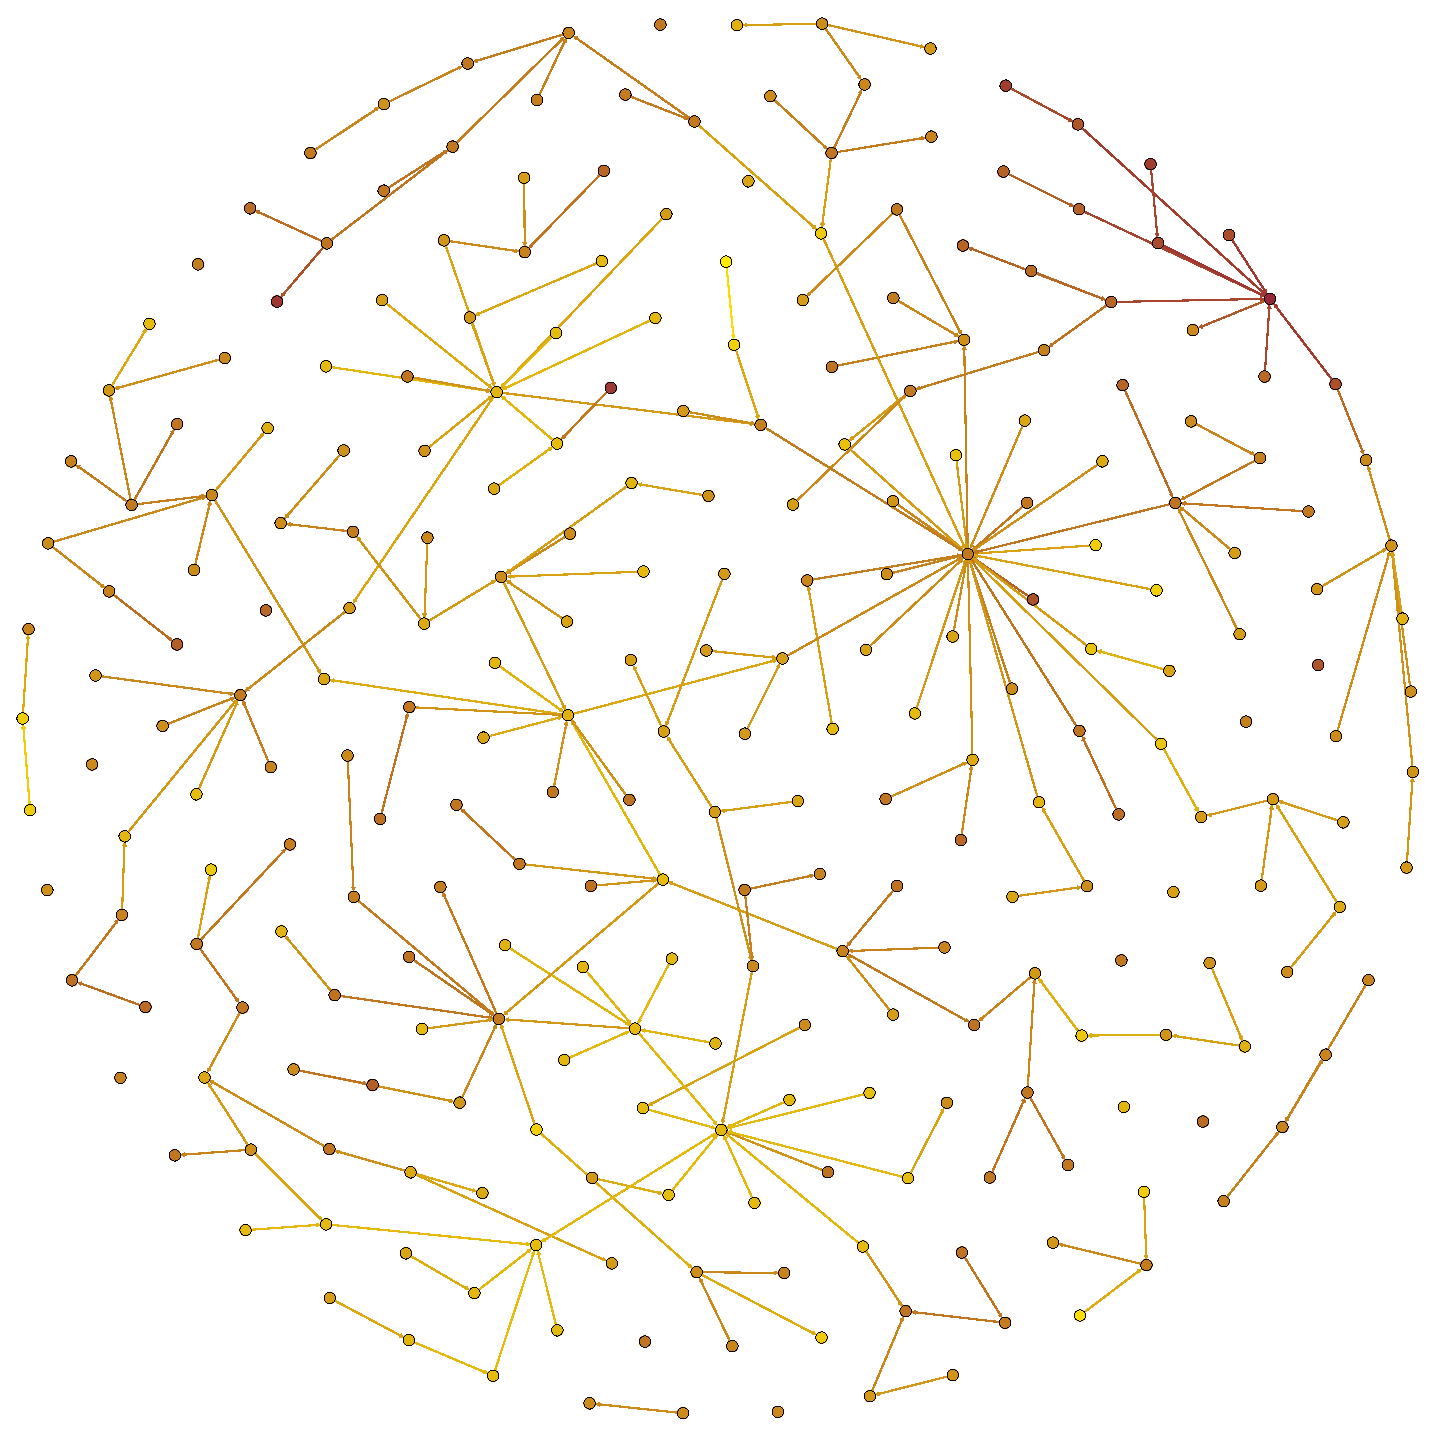
\includegraphics[scale=0.7]{figures/clustering.eps}

    Our classifier is trained on a set of 2035 manually annotated
    papers where some authors have been identified. We randomly
    generate positive and negative training pairs of example
    papers to train a Support Vector Machine with linear kernel.
}

\column{0.33}
\block{Relevance estimation}{
    Lorem ipsum

    Lorem ipsum


    Lorem ipsum

    Lorem ipsum
}
\block{Results}{
    Lorem ipsum

    Lorem ipsum


    Lorem ipsum

    Lorem ipsum
}
\block{References}{
    Lorem ipsum

    Lorem ipsum


    Lorem ipsum

    Lorem ipsum
}





\end{columns}


\end{document}
